\documentclass[12pt,a4paper]{article}
\usepackage[top=1.5cm, bottom=1.5cm, left=2.0cm, right=1.5cm] {geometry}
\usepackage{amsmath,amssymb,txfonts}
\usepackage{tkz-euclide}
\usepackage{setspace}
\usepackage{lastpage}

\usepackage{tikz,tkz-tab}
%\usepackage[solcolor]{ex_test}
\usepackage[dethi]{ex_test} % Chỉ hiển thị đề thi
%\usepackage[loigiai]{ex_test} % Hiển thị lời giải
%\usepackage[color]{ex_test} % Khoanh các đáp án
\usetikzlibrary{shapes.geometric,arrows,calc,intersections,angles,quotes,patterns,snakes,positioning}
\everymath{\displaystyle}

\def\colorEX{\color{purple}}
%\def\colorEX{}%Không tô màu đáp án đúng trong tùy chọn loigiai
\renewtheorem{ex}{\color{violet}Câu}
\renewcommand{\FalseEX}{\stepcounter{dapan}{{\bf \textcolor{blue}{\Alph{dapan}.}}}}
\renewcommand{\TrueEX}{\stepcounter{dapan}{{\bf \textcolor{blue}{\Alph{dapan}.}}}}

%---------- Khai báo viết tắt, in đáp án
\newcommand{\hoac}[1]{ %hệ hoặc
    \left[\begin{aligned}#1\end{aligned}\right.}
\newcommand{\heva}[1]{ %hệ và
    \left\{\begin{aligned}#1\end{aligned}\right.}

%Tiêu đề
\newcommand{\tenso}{}
\newcommand{\tentruong}{}
\newcommand{\tenkythi}{ĐỀ ÔN TẬP}
\newcommand{\tenmonthi}{Môn học: }
\newcommand{\thoigian}{}
\newcommand{\tieude}[1]{
    \noindent
     \begin{minipage}[b]{6cm}
    \centerline{\textbf{\fontsize{11}{0}\selectfont \tenso}}
    \centerline{\fontsize{11}{0}\selectfont \tentruong}  
  \end{minipage}\hspace{1cm}
  \begin{minipage}[b]{11cm}
    \centerline{\textbf{\fontsize{11}{0}\selectfont \tenkythi}}
    \centerline{\textbf{\fontsize{11}{0}\selectfont \tenmonthi}}
    \centerline{\textit{\fontsize{11}{0}\selectfont Thời \underline{gian làm bài: \thoigian  } phút }}
  \end{minipage}
  \vspace*{3mm}
  \noindent
  \begin{minipage}[t]{12cm}
    \textbf{Họ, tên thí sinh:}\dotfill\\
    \textbf{Số báo danh:}\dotfill
  \end{minipage}\hfill
  \begin{minipage}[b]{3cm}
    \setlength\fboxrule{1pt}
    \setlength\fboxsep{3pt}
    \vspace*{3mm}\fbox{\bf Mã đề thi #1}
  \end{minipage}\\
}

\newcommand{\chantrang}[2]{\rfoot{Trang \thepage $-$ Mã đề #2}}
\pagestyle{fancy}
\fancyhf{}
\renewcommand{\headrulewidth}{0pt} 
\renewcommand{\footrulewidth}{0pt}

\begin{document}
%Thiết lập giãn dọng 1.5cm 
%\setlength{\lineskip}{1.5em}



%Nội dung trắc nghiệm bắt đầu ở đây


\tieude{001}
\chantrang{\pageref{LastPage}}{001}
\setcounter{page}{1}
{\bf PHẦN I. Câu trắc nghiệm nhiều phương án lựa chọn.}
\setcounter{ex}{0}
\Opensolutionfile{ans}[ans/ans001-1]
\begin{ex}
 Cho hình chóp ${S.BCEF}$ có đáy là hình chữ nhật tâm ${I}$. Gọi ${P,Q}$ lần lượt là các điểm thuộc các cạnh ${SB,SC}$ sao cho $PB=4SP, SC=5SQ$. Khẳng định nào sau đây là khẳng định đúng? 
\begin{center}
 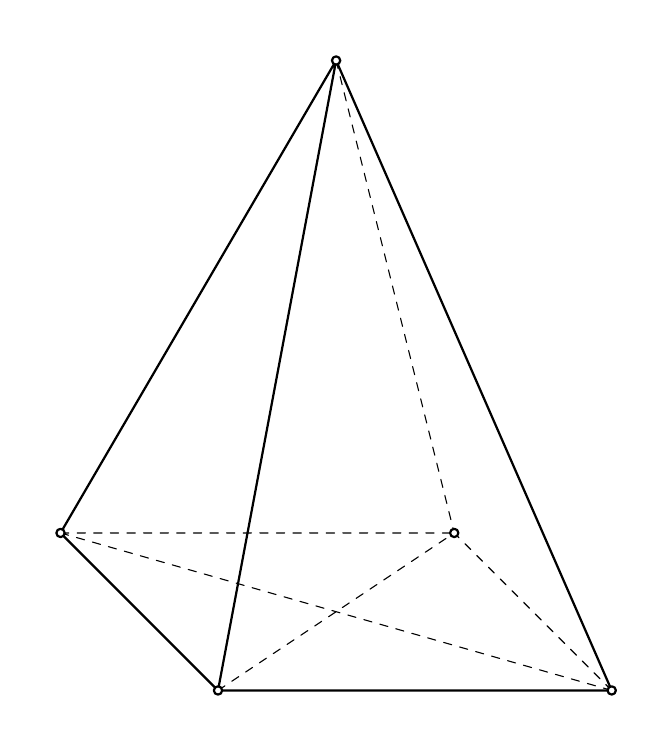
\begin{tikzpicture}[line join=round, line cap=round,thick]
\coordinate (B) at (0,0);
\coordinate (C) at (2,-2);
\coordinate (F) at (5,0);
\coordinate (E) at ($(C)+(F)-(B)$);
\coordinate (O) at ($(B)!0.5!(E)$);
\coordinate (S) at ($(O)+(0,7)$);
\draw(S)--(B) (S)--(C) (S)--(E) (B)--(C) (C)--(E);
\draw[dashed,thin](B)--(E) (B)--(F) (E)--(F) (S)--(F) (C)--(F);
\foreach \i/\g in {S/90,B/180,C/-90,E/-90,F/0}{\draw[fill=white](\i) circle (1.5pt) ($(\i)+(\g:3mm)$) node[scale=1]{};}
\end{tikzpicture}

\end{center}
\choice
{ ${PE}$ // ${SC}$ }
   { ${BQ}$ // ${CF}$ }
     { ${IP}$ // ${SB}$ }
    { \True ${PQ}$ // ${EF}$ }
\loigiai{\begin{center}
 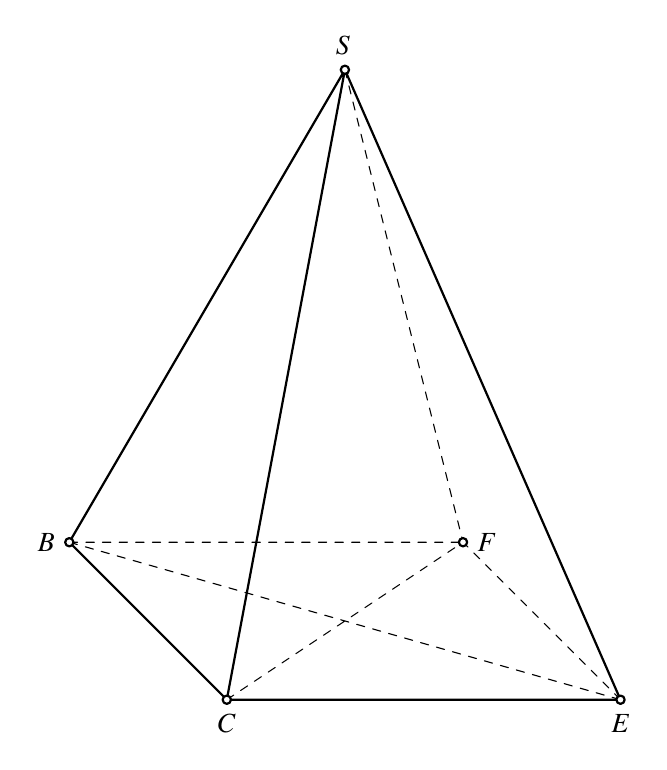
\begin{tikzpicture}[line join=round, line cap=round,thick]
\coordinate (B) at (0,0);
\coordinate (C) at (2,-2);
\coordinate (F) at (5,0);
\coordinate (E) at ($(C)+(F)-(B)$);
\coordinate (O) at ($(B)!0.5!(E)$);
\coordinate (S) at ($(O)+(0,7)$);
\draw(S)--(B) (S)--(C) (S)--(E) (B)--(C) (C)--(E);
\draw[dashed,thin](B)--(E) (B)--(F) (E)--(F) (S)--(F) (C)--(F);
\foreach \i/\g in {S/90,B/180,C/-90,E/-90,F/0}{\draw[fill=white](\i) circle (1.5pt) ($(\i)+(\g:3mm)$) node[scale=1]{$\i$};}
\end{tikzpicture}

\end{center}
 
 $\dfrac{SP}{SB}=\dfrac{SQ}{SC}=\frac{1}{5}\Rightarrow PQ$ // ${BC}$ // ${EF}$. 
 }\end{ex}

\begin{ex}
 Cho hình chóp ${S.BCEF}$ có đáy là hình thoi tâm ${O}$. Gọi ${M,N}$ lần lượt là các điểm thuộc các đoạn thẳng ${SC,CF}$ sao cho $CM=4SM, CN=4NF$. Khẳng định nào sau đây là khẳng định đúng? 
\begin{center}
 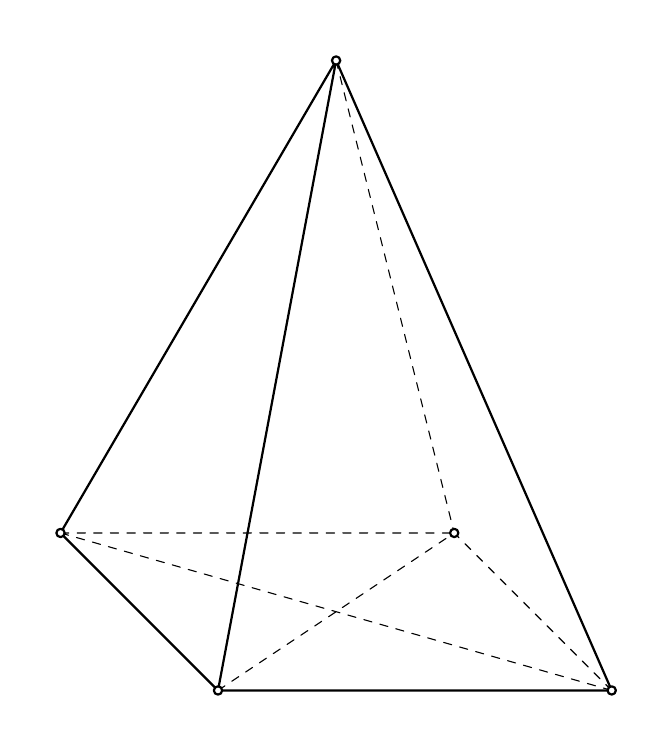
\begin{tikzpicture}[line join=round, line cap=round,thick]
\coordinate (B) at (0,0);
\coordinate (C) at (2,-2);
\coordinate (F) at (5,0);
\coordinate (E) at ($(C)+(F)-(B)$);
\coordinate (O) at ($(B)!0.5!(E)$);
\coordinate (S) at ($(O)+(0,7)$);
\draw(S)--(B) (S)--(C) (S)--(E) (B)--(C) (C)--(E);
\draw[dashed,thin](B)--(E) (B)--(F) (E)--(F) (S)--(F) (C)--(F);
\foreach \i/\g in {S/90,B/180,C/-90,E/-90,F/0}{\draw[fill=white](\i) circle (1.5pt) ($(\i)+(\g:3mm)$) node[scale=1]{};}
\end{tikzpicture}

\end{center}
\choice
{ ${BN}$ // ${CF}$ }
   { ${MN}$ // ${CE}$ }
     { \True ${SF}$  // ${MN}$ }
    { ${MF}$ // ${EN}$ }
\loigiai{\begin{center}
 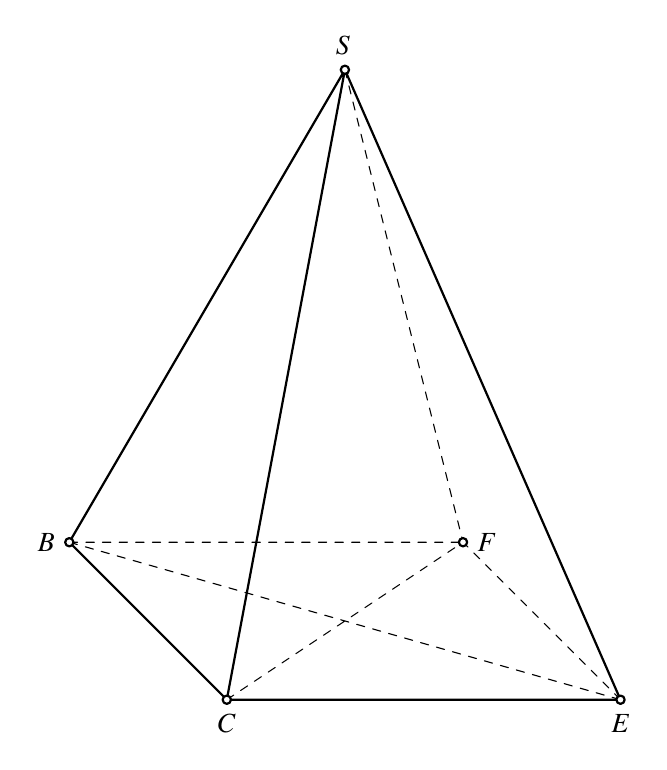
\begin{tikzpicture}[line join=round, line cap=round,thick]
\coordinate (B) at (0,0);
\coordinate (C) at (2,-2);
\coordinate (F) at (5,0);
\coordinate (E) at ($(C)+(F)-(B)$);
\coordinate (O) at ($(B)!0.5!(E)$);
\coordinate (S) at ($(O)+(0,7)$);
\draw(S)--(B) (S)--(C) (S)--(E) (B)--(C) (C)--(E);
\draw[dashed,thin](B)--(E) (B)--(F) (E)--(F) (S)--(F) (C)--(F);
\foreach \i/\g in {S/90,B/180,C/-90,E/-90,F/0}{\draw[fill=white](\i) circle (1.5pt) ($(\i)+(\g:3mm)$) node[scale=1]{$\i$};}
\end{tikzpicture}

\end{center}
 
 $\dfrac{CM}{SC}=\dfrac{CN}{CF}=\frac{4}{5}\Rightarrow MN$ // ${SF}$. 
 }\end{ex}

\begin{ex}
 Cho hình chóp ${S.BCEF}$ có đáy là hình thoi tâm ${I}$. Gọi ${M,N}$ lần lượt là các trung điểm của ${BC,EF}$ và ${G,K}$ lần lượt là trọng tâm các tam giác ${SBC,SEF}$. Khẳng định nào sau đây là khẳng định đúng? 
\begin{center}
 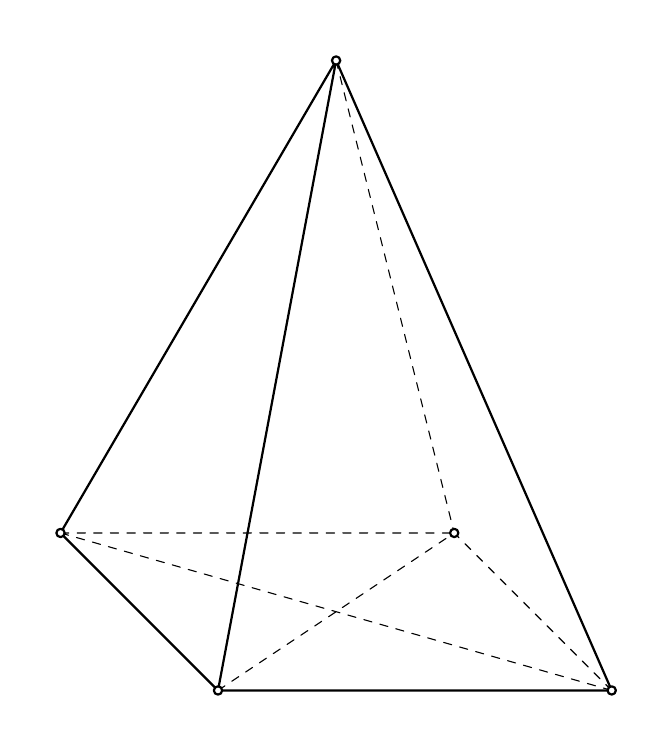
\begin{tikzpicture}[line join=round, line cap=round,thick]
\coordinate (B) at (0,0);
\coordinate (C) at (2,-2);
\coordinate (F) at (5,0);
\coordinate (E) at ($(C)+(F)-(B)$);
\coordinate (O) at ($(B)!0.5!(E)$);
\coordinate (S) at ($(O)+(0,7)$);
\draw(S)--(B) (S)--(C) (S)--(E) (B)--(C) (C)--(E);
\draw[dashed,thin](B)--(E) (B)--(F) (E)--(F) (S)--(F) (C)--(F);
\foreach \i/\g in {S/90,B/180,C/-90,E/-90,F/0}{\draw[fill=white](\i) circle (1.5pt) ($(\i)+(\g:3mm)$) node[scale=1]{};}
\end{tikzpicture}

\end{center}
\choice
{ ${KM}$ // ${CN}$ }
   { \True ${ME}$  // ${BN}$ }
     { ${IK}$ // ${SM}$ }
    { ${GK}$ // ${EF}$ }
\loigiai{\begin{center}
 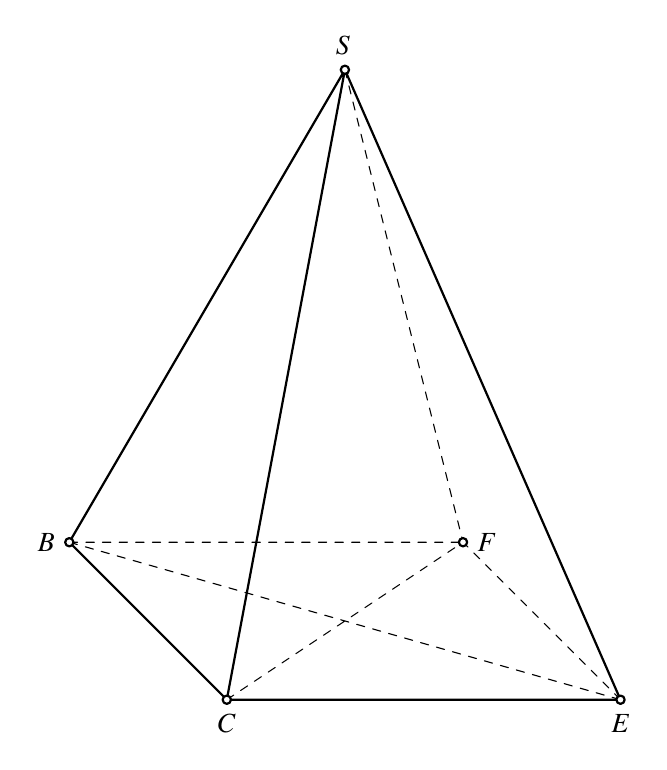
\begin{tikzpicture}[line join=round, line cap=round,thick]
\coordinate (B) at (0,0);
\coordinate (C) at (2,-2);
\coordinate (F) at (5,0);
\coordinate (E) at ($(C)+(F)-(B)$);
\coordinate (O) at ($(B)!0.5!(E)$);
\coordinate (S) at ($(O)+(0,7)$);
\draw(S)--(B) (S)--(C) (S)--(E) (B)--(C) (C)--(E);
\draw[dashed,thin](B)--(E) (B)--(F) (E)--(F) (S)--(F) (C)--(F);
\foreach \i/\g in {S/90,B/180,C/-90,E/-90,F/0}{\draw[fill=white](\i) circle (1.5pt) ($(\i)+(\g:3mm)$) node[scale=1]{$\i$};}
\end{tikzpicture}

\end{center}
 
 ${FM}$  // ${CN}$ là khẳng định đúng. 
 }\end{ex}

\begin{ex}
 Cho hình chóp ${S.ABEF}$ có đáy là hình chữ nhật tâm ${O}$. Gọi ${M,Q}$ lần lượt là các điểm thuộc các cạnh ${SA,SB}$ sao cho $SA=4SM, QB=3SQ$. Khẳng định nào sau đây là khẳng định đúng? 
\begin{center}
 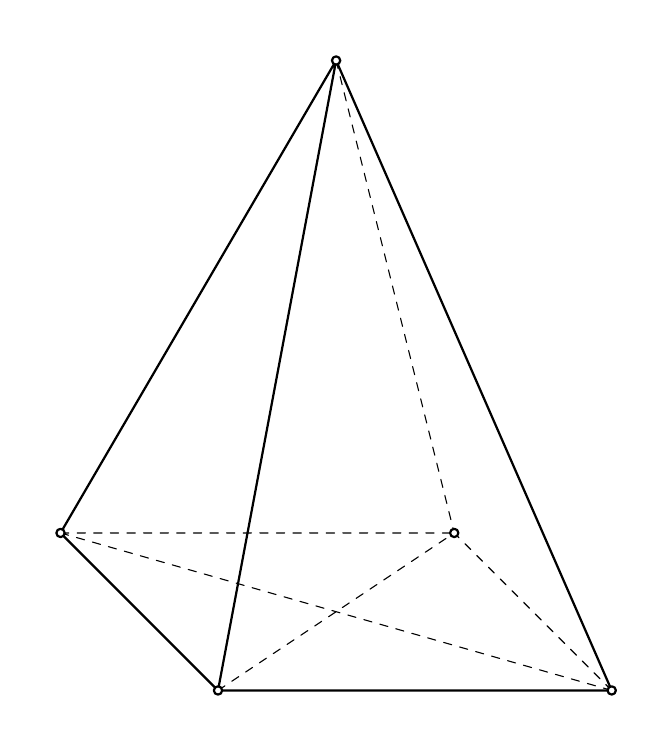
\begin{tikzpicture}[line join=round, line cap=round,thick]
\coordinate (A) at (0,0);
\coordinate (B) at (2,-2);
\coordinate (F) at (5,0);
\coordinate (E) at ($(B)+(F)-(A)$);
\coordinate (O) at ($(A)!0.5!(E)$);
\coordinate (S) at ($(O)+(0,7)$);
\draw(S)--(A) (S)--(B) (S)--(E) (A)--(B) (B)--(E);
\draw[dashed,thin](A)--(E) (A)--(F) (E)--(F) (S)--(F) (B)--(F);
\foreach \i/\g in {S/90,A/180,B/-90,E/-90,F/0}{\draw[fill=white](\i) circle (1.5pt) ($(\i)+(\g:3mm)$) node[scale=1]{};}
\end{tikzpicture}

\end{center}
\choice
{ ${FQ}$ // ${EM}$ }
   { ${AQ}$ // ${BF}$ }
     { ${OQ}$ // ${SE}$ }
    { \True ${MQ}$ // ${AB}$ }
\loigiai{\begin{center}
 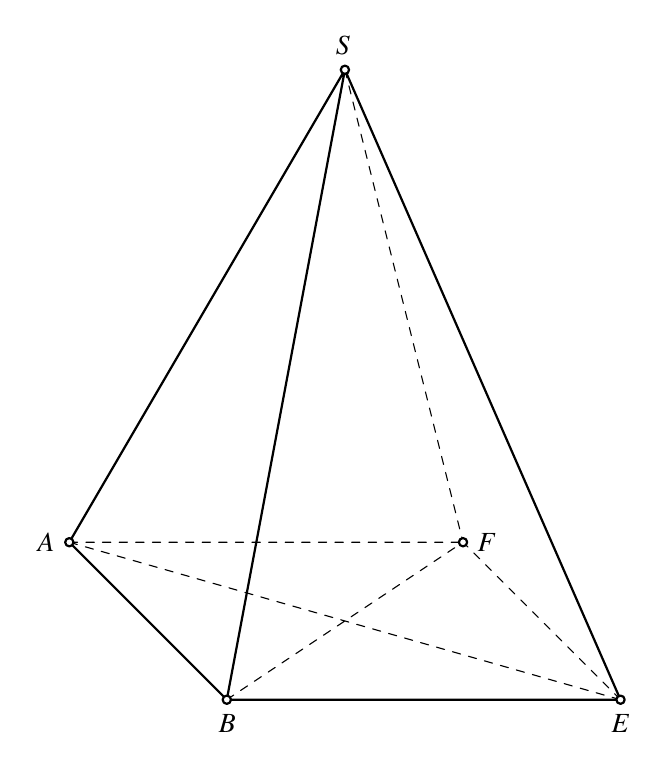
\begin{tikzpicture}[line join=round, line cap=round,thick]
\coordinate (A) at (0,0);
\coordinate (B) at (2,-2);
\coordinate (F) at (5,0);
\coordinate (E) at ($(B)+(F)-(A)$);
\coordinate (O) at ($(A)!0.5!(E)$);
\coordinate (S) at ($(O)+(0,7)$);
\draw(S)--(A) (S)--(B) (S)--(E) (A)--(B) (B)--(E);
\draw[dashed,thin](A)--(E) (A)--(F) (E)--(F) (S)--(F) (B)--(F);
\foreach \i/\g in {S/90,A/180,B/-90,E/-90,F/0}{\draw[fill=white](\i) circle (1.5pt) ($(\i)+(\g:3mm)$) node[scale=1]{$\i$};}
\end{tikzpicture}

\end{center}
 
 $\dfrac{SM}{SA}=\dfrac{SQ}{SB}=\frac{1}{4}\Rightarrow MQ$ // ${AB}$ // ${EF}$. 
 }\end{ex}

\begin{ex}
 Cho hình chóp ${S.ABEF}$ có đáy là hình chữ nhật tâm ${O}$. Gọi ${P,N}$ lần lượt là các điểm thuộc các cạnh ${SA,SB}$ sao cho $PA=3SP, SB=4SN$. Khẳng định nào sau đây là khẳng định đúng? 
\begin{center}
 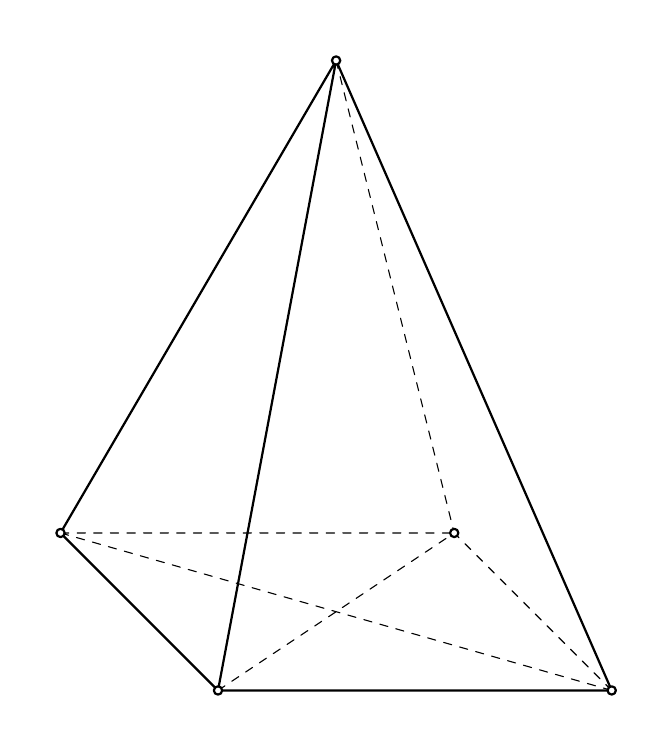
\begin{tikzpicture}[line join=round, line cap=round,thick]
\coordinate (A) at (0,0);
\coordinate (B) at (2,-2);
\coordinate (F) at (5,0);
\coordinate (E) at ($(B)+(F)-(A)$);
\coordinate (O) at ($(A)!0.5!(E)$);
\coordinate (S) at ($(O)+(0,7)$);
\draw(S)--(A) (S)--(B) (S)--(E) (A)--(B) (B)--(E);
\draw[dashed,thin](A)--(E) (A)--(F) (E)--(F) (S)--(F) (B)--(F);
\foreach \i/\g in {S/90,A/180,B/-90,E/-90,F/0}{\draw[fill=white](\i) circle (1.5pt) ($(\i)+(\g:3mm)$) node[scale=1]{};}
\end{tikzpicture}

\end{center}
\choice
{ ${OP}$ // ${SA}$ }
   { \True ${PN}$ // ${EF}$ }
     { ${OP}$ // ${SE}$ }
    { ${ON}$ // ${SF}$ }
\loigiai{\begin{center}
 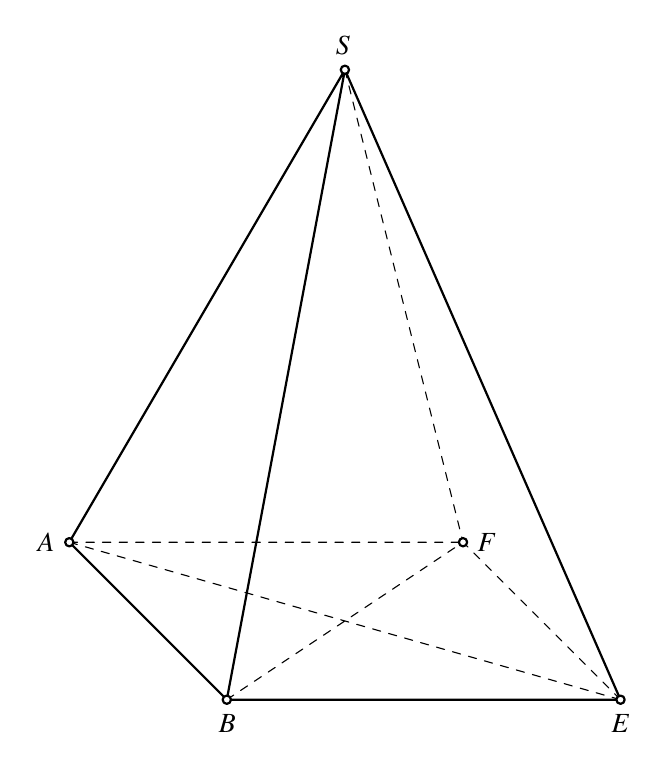
\begin{tikzpicture}[line join=round, line cap=round,thick]
\coordinate (A) at (0,0);
\coordinate (B) at (2,-2);
\coordinate (F) at (5,0);
\coordinate (E) at ($(B)+(F)-(A)$);
\coordinate (O) at ($(A)!0.5!(E)$);
\coordinate (S) at ($(O)+(0,7)$);
\draw(S)--(A) (S)--(B) (S)--(E) (A)--(B) (B)--(E);
\draw[dashed,thin](A)--(E) (A)--(F) (E)--(F) (S)--(F) (B)--(F);
\foreach \i/\g in {S/90,A/180,B/-90,E/-90,F/0}{\draw[fill=white](\i) circle (1.5pt) ($(\i)+(\g:3mm)$) node[scale=1]{$\i$};}
\end{tikzpicture}

\end{center}
 
 $\dfrac{SP}{SA}=\dfrac{SN}{SB}=\frac{1}{4}\Rightarrow PN$ // ${AB}$ // ${EF}$. 
 }\end{ex}

\begin{ex}
 Cho hình chóp ${S.ABCE}$ có đáy là hình thoi tâm ${O}$. Gọi ${P,Q}$ lần lượt là các điểm thuộc các cạnh ${SA,SB}$ sao cho $SA=3SP, QB=2SQ$. Khẳng định nào sau đây là khẳng định đúng? 
\begin{center}
 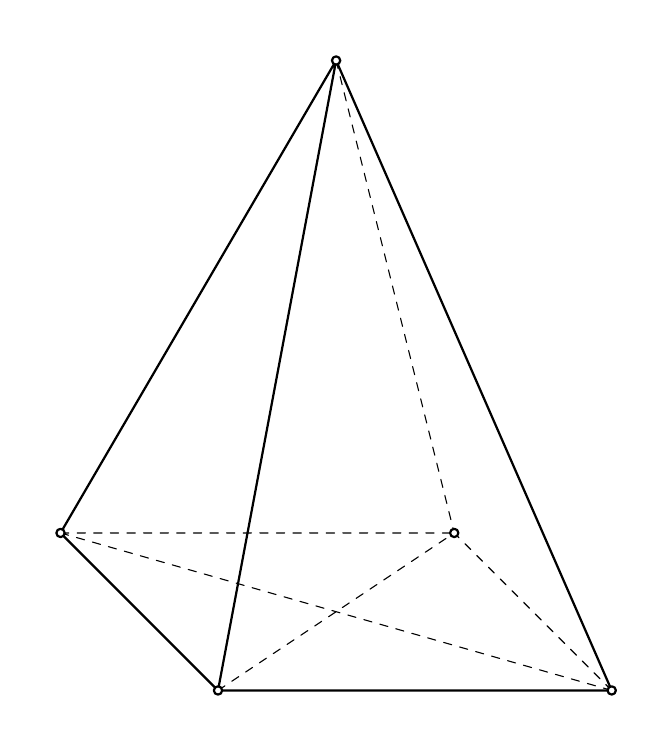
\begin{tikzpicture}[line join=round, line cap=round,thick]
\coordinate (A) at (0,0);
\coordinate (B) at (2,-2);
\coordinate (E) at (5,0);
\coordinate (C) at ($(B)+(E)-(A)$);
\coordinate (O) at ($(A)!0.5!(C)$);
\coordinate (S) at ($(O)+(0,7)$);
\draw(S)--(A) (S)--(B) (S)--(C) (A)--(B) (B)--(C);
\draw[dashed,thin](A)--(C) (A)--(E) (C)--(E) (S)--(E) (B)--(E);
\foreach \i/\g in {S/90,A/180,B/-90,C/-90,E/0}{\draw[fill=white](\i) circle (1.5pt) ($(\i)+(\g:3mm)$) node[scale=1]{};}
\end{tikzpicture}

\end{center}
\choice
{ ${AQ}$ // ${BE}$ }
   { ${PQ}$ // ${BC}$ }
     { \True ${CE}$ // ${PQ}$ }
    { ${OP}$ // ${SC}$ }
\loigiai{\begin{center}
 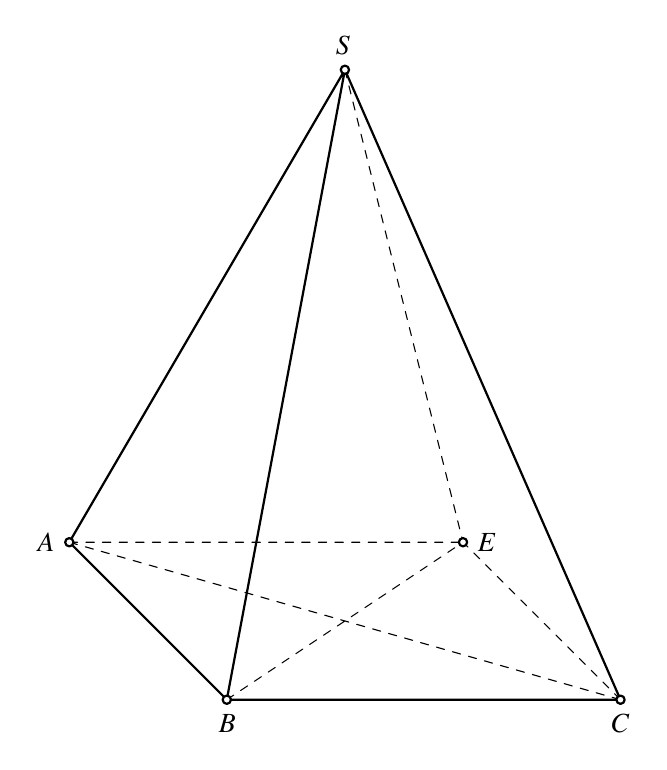
\begin{tikzpicture}[line join=round, line cap=round,thick]
\coordinate (A) at (0,0);
\coordinate (B) at (2,-2);
\coordinate (E) at (5,0);
\coordinate (C) at ($(B)+(E)-(A)$);
\coordinate (O) at ($(A)!0.5!(C)$);
\coordinate (S) at ($(O)+(0,7)$);
\draw(S)--(A) (S)--(B) (S)--(C) (A)--(B) (B)--(C);
\draw[dashed,thin](A)--(C) (A)--(E) (C)--(E) (S)--(E) (B)--(E);
\foreach \i/\g in {S/90,A/180,B/-90,C/-90,E/0}{\draw[fill=white](\i) circle (1.5pt) ($(\i)+(\g:3mm)$) node[scale=1]{$\i$};}
\end{tikzpicture}

\end{center}
 
 $\dfrac{SP}{SA}=\dfrac{SQ}{SB}=\frac{1}{3}\Rightarrow PQ$ // ${AB}$ // ${CE}$. 
 }\end{ex}

\begin{ex}
 Cho hình chóp ${S.BCEF}$ có đáy là hình vuông tâm ${J}$. Gọi ${M,H}$ lần lượt là các điểm thuộc các cạnh ${SB,SC}$ sao cho $SB=5SM, HC=4SH$. Khẳng định nào sau đây là khẳng định đúng? 
\begin{center}
 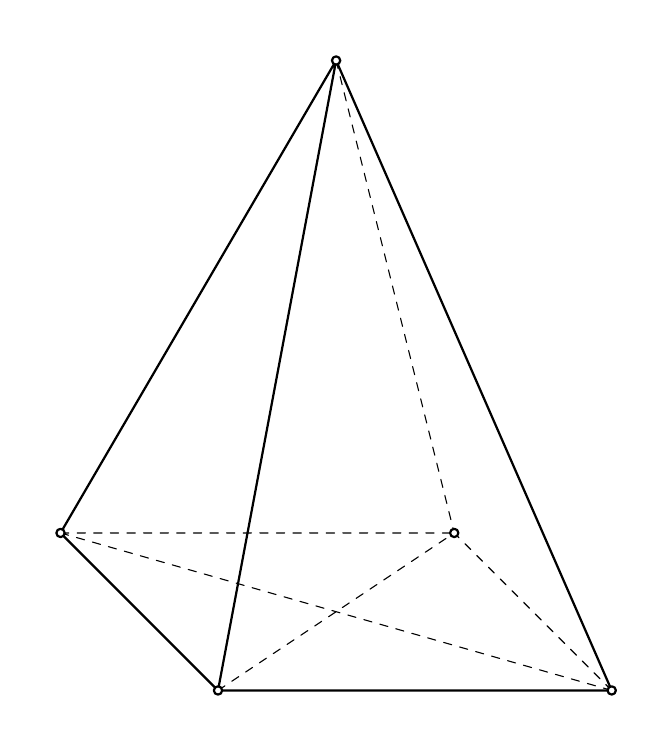
\begin{tikzpicture}[line join=round, line cap=round,thick]
\coordinate (B) at (0,0);
\coordinate (C) at (2,-2);
\coordinate (F) at (5,0);
\coordinate (E) at ($(C)+(F)-(B)$);
\coordinate (O) at ($(B)!0.5!(E)$);
\coordinate (S) at ($(O)+(0,7)$);
\draw(S)--(B) (S)--(C) (S)--(E) (B)--(C) (C)--(E);
\draw[dashed,thin](B)--(E) (B)--(F) (E)--(F) (S)--(F) (C)--(F);
\foreach \i/\g in {S/90,B/180,C/-90,E/-90,F/0}{\draw[fill=white](\i) circle (1.5pt) ($(\i)+(\g:3mm)$) node[scale=1]{};}
\end{tikzpicture}

\end{center}
\choice
{ ${MH}$ // ${CE}$ }
   { ${BH}$ // ${CF}$ }
     { ${FH}$ // ${EM}$ }
    { \True ${MH}$ // ${BC}$ }
\loigiai{\begin{center}
 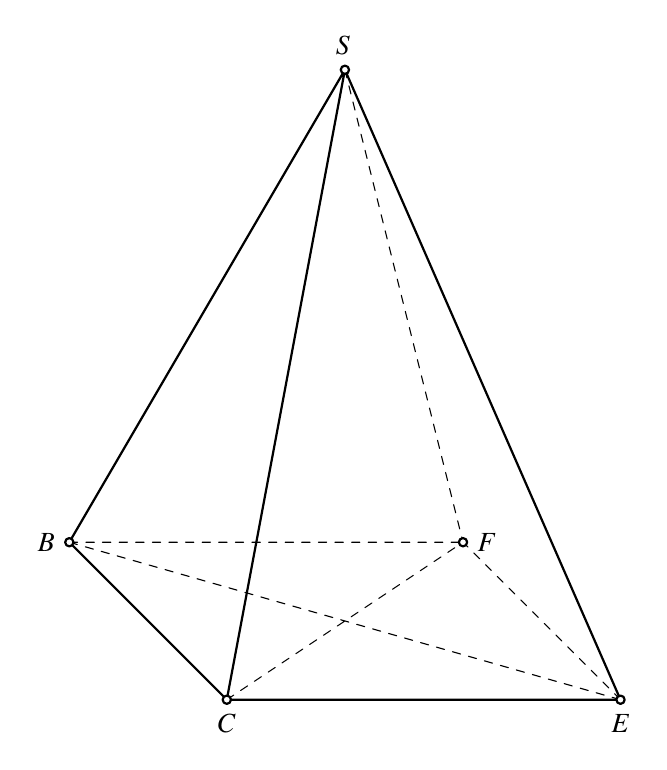
\begin{tikzpicture}[line join=round, line cap=round,thick]
\coordinate (B) at (0,0);
\coordinate (C) at (2,-2);
\coordinate (F) at (5,0);
\coordinate (E) at ($(C)+(F)-(B)$);
\coordinate (O) at ($(B)!0.5!(E)$);
\coordinate (S) at ($(O)+(0,7)$);
\draw(S)--(B) (S)--(C) (S)--(E) (B)--(C) (C)--(E);
\draw[dashed,thin](B)--(E) (B)--(F) (E)--(F) (S)--(F) (C)--(F);
\foreach \i/\g in {S/90,B/180,C/-90,E/-90,F/0}{\draw[fill=white](\i) circle (1.5pt) ($(\i)+(\g:3mm)$) node[scale=1]{$\i$};}
\end{tikzpicture}

\end{center}
 
 $\dfrac{SM}{SB}=\dfrac{SH}{SC}=\frac{1}{5}\Rightarrow MH$ // ${BC}$ // ${EF}$. 
 }\end{ex}

\begin{ex}
 Cho hình chóp ${S.ABCE}$ có đáy là hình chữ nhật tâm ${J}$. Gọi ${G,H}$ lần lượt là các điểm thuộc các cạnh ${SA,SB}$ sao cho $GA=3SG, SB=4SH$. Khẳng định nào sau đây là khẳng định đúng? 
\begin{center}
 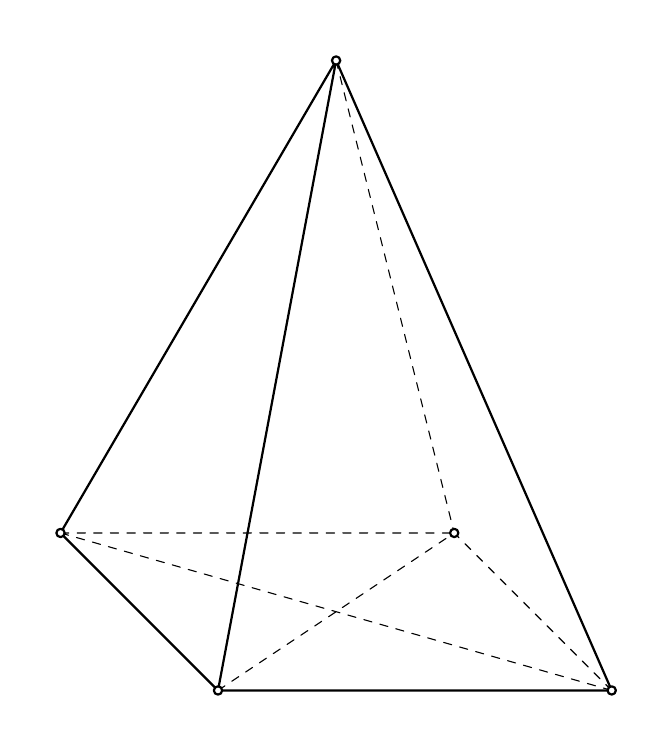
\begin{tikzpicture}[line join=round, line cap=round,thick]
\coordinate (A) at (0,0);
\coordinate (B) at (2,-2);
\coordinate (E) at (5,0);
\coordinate (C) at ($(B)+(E)-(A)$);
\coordinate (O) at ($(A)!0.5!(C)$);
\coordinate (S) at ($(O)+(0,7)$);
\draw(S)--(A) (S)--(B) (S)--(C) (A)--(B) (B)--(C);
\draw[dashed,thin](A)--(C) (A)--(E) (C)--(E) (S)--(E) (B)--(E);
\foreach \i/\g in {S/90,A/180,B/-90,C/-90,E/0}{\draw[fill=white](\i) circle (1.5pt) ($(\i)+(\g:3mm)$) node[scale=1]{};}
\end{tikzpicture}

\end{center}
\choice
{ ${JH}$ // ${SE}$ }
   { \True ${GH}$ // ${CE}$ }
     { ${JG}$ // ${SA}$ }
    { ${EH}$ // ${CG}$ }
\loigiai{\begin{center}
 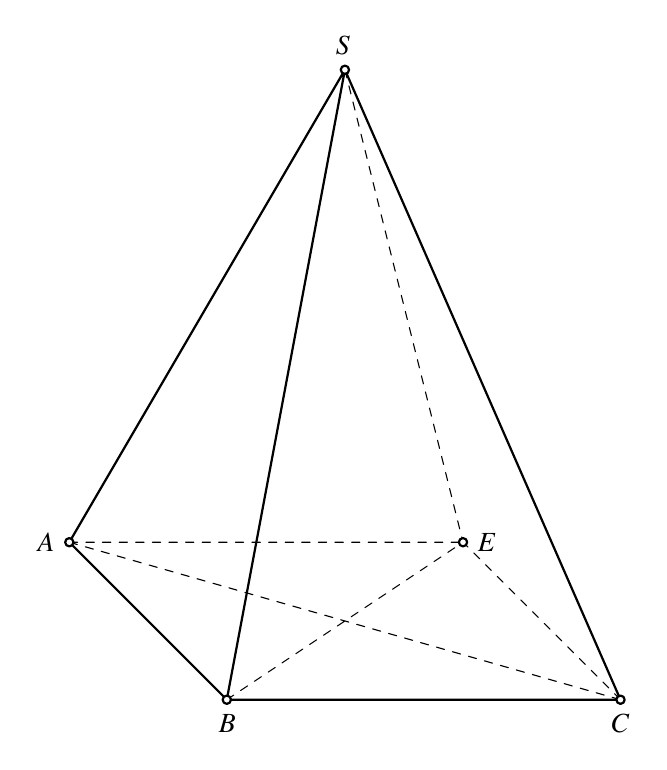
\begin{tikzpicture}[line join=round, line cap=round,thick]
\coordinate (A) at (0,0);
\coordinate (B) at (2,-2);
\coordinate (E) at (5,0);
\coordinate (C) at ($(B)+(E)-(A)$);
\coordinate (O) at ($(A)!0.5!(C)$);
\coordinate (S) at ($(O)+(0,7)$);
\draw(S)--(A) (S)--(B) (S)--(C) (A)--(B) (B)--(C);
\draw[dashed,thin](A)--(C) (A)--(E) (C)--(E) (S)--(E) (B)--(E);
\foreach \i/\g in {S/90,A/180,B/-90,C/-90,E/0}{\draw[fill=white](\i) circle (1.5pt) ($(\i)+(\g:3mm)$) node[scale=1]{$\i$};}
\end{tikzpicture}

\end{center}
 
 $\dfrac{SG}{SA}=\dfrac{SH}{SB}=\frac{1}{4}\Rightarrow GH$ // ${AB}$ // ${CE}$. 
 }\end{ex}

\begin{ex}
 Cho hình chóp ${S.BCDE}$ có đáy là hình bình hành tâm ${O}$. Gọi ${P,N}$ lần lượt là các điểm thuộc các cạnh ${SB,SC}$ sao cho $SB=4SP, NC=3SN$. Khẳng định nào sau đây là khẳng định đúng? 
\begin{center}
 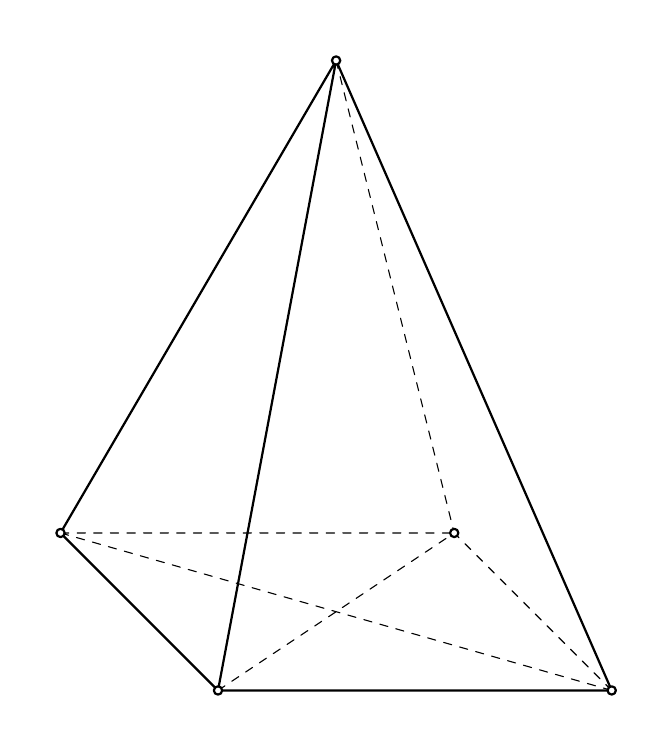
\begin{tikzpicture}[line join=round, line cap=round,thick]
\coordinate (B) at (0,0);
\coordinate (C) at (2,-2);
\coordinate (E) at (5,0);
\coordinate (D) at ($(C)+(E)-(B)$);
\coordinate (O) at ($(B)!0.5!(D)$);
\coordinate (S) at ($(O)+(0,7)$);
\draw(S)--(B) (S)--(C) (S)--(D) (B)--(C) (C)--(D);
\draw[dashed,thin](B)--(D) (B)--(E) (D)--(E) (S)--(E) (C)--(E);
\foreach \i/\g in {S/90,B/180,C/-90,D/-90,E/0}{\draw[fill=white](\i) circle (1.5pt) ($(\i)+(\g:3mm)$) node[scale=1]{};}
\end{tikzpicture}

\end{center}
\choice
{ \True ${BC}$  // ${PN}$ }
   { ${PE}$ // ${DN}$ }
     { ${BN}$ // ${CE}$ }
    { ${ON}$ // ${SE}$ }
\loigiai{\begin{center}
 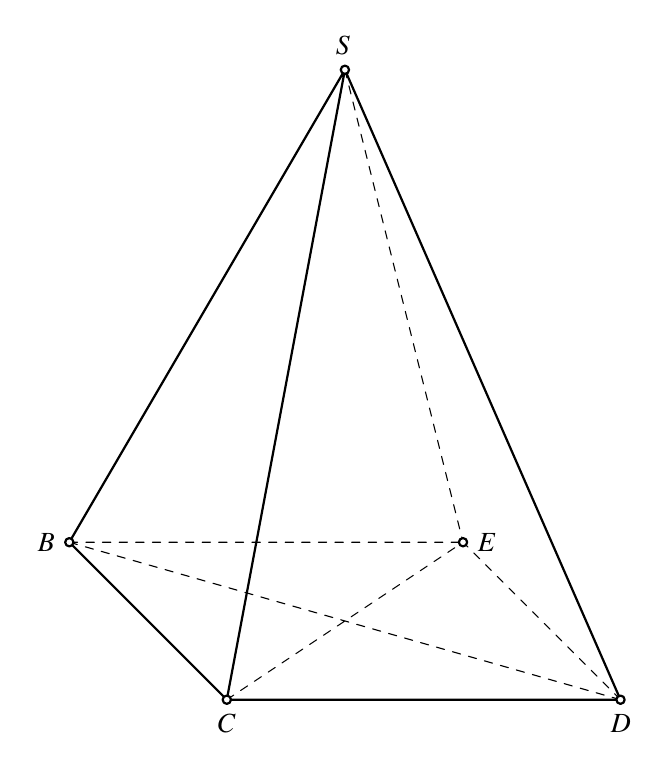
\begin{tikzpicture}[line join=round, line cap=round,thick]
\coordinate (B) at (0,0);
\coordinate (C) at (2,-2);
\coordinate (E) at (5,0);
\coordinate (D) at ($(C)+(E)-(B)$);
\coordinate (O) at ($(B)!0.5!(D)$);
\coordinate (S) at ($(O)+(0,7)$);
\draw(S)--(B) (S)--(C) (S)--(D) (B)--(C) (C)--(D);
\draw[dashed,thin](B)--(D) (B)--(E) (D)--(E) (S)--(E) (C)--(E);
\foreach \i/\g in {S/90,B/180,C/-90,D/-90,E/0}{\draw[fill=white](\i) circle (1.5pt) ($(\i)+(\g:3mm)$) node[scale=1]{$\i$};}
\end{tikzpicture}

\end{center}
 
 $\dfrac{SP}{SB}=\dfrac{SN}{SC}=\frac{1}{4}\Rightarrow PN$ // ${BC}$ // ${DE}$. 
 }\end{ex}

\begin{ex}
 Cho hình chóp ${S.ABEF}$ có đáy là hình chữ nhật tâm ${I}$. Gọi ${G,Q}$ lần lượt là các điểm thuộc các cạnh ${SA,SB}$ sao cho $SA=4SG, QB=3SQ$. Khẳng định nào sau đây là khẳng định đúng? 
\begin{center}
 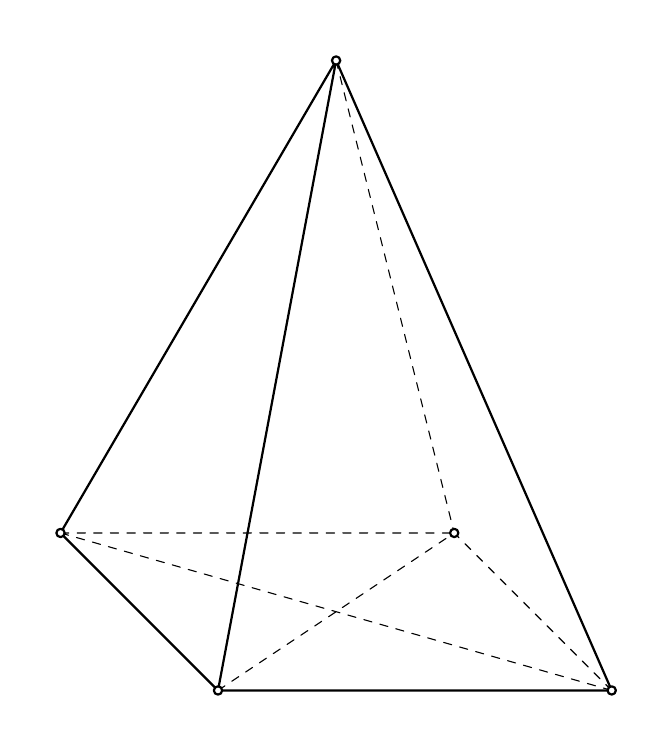
\begin{tikzpicture}[line join=round, line cap=round,thick]
\coordinate (A) at (0,0);
\coordinate (B) at (2,-2);
\coordinate (F) at (5,0);
\coordinate (E) at ($(B)+(F)-(A)$);
\coordinate (O) at ($(A)!0.5!(E)$);
\coordinate (S) at ($(O)+(0,7)$);
\draw(S)--(A) (S)--(B) (S)--(E) (A)--(B) (B)--(E);
\draw[dashed,thin](A)--(E) (A)--(F) (E)--(F) (S)--(F) (B)--(F);
\foreach \i/\g in {S/90,A/180,B/-90,E/-90,F/0}{\draw[fill=white](\i) circle (1.5pt) ($(\i)+(\g:3mm)$) node[scale=1]{};}
\end{tikzpicture}

\end{center}
\choice
{ ${FQ}$ // ${EG}$ }
   { ${IQ}$ // ${SF}$ }
     { \True ${EF}$ // ${GQ}$ }
    { ${IG}$ // ${SE}$ }
\loigiai{\begin{center}
 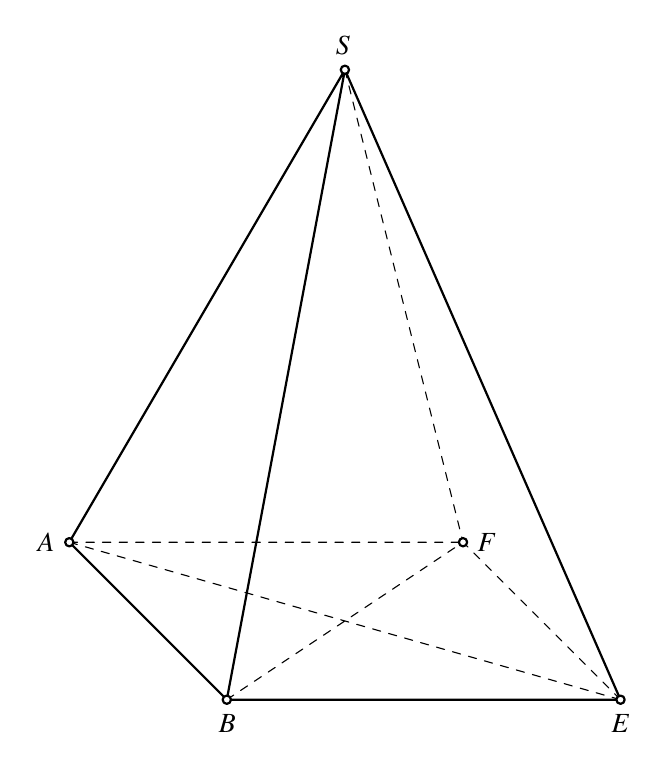
\begin{tikzpicture}[line join=round, line cap=round,thick]
\coordinate (A) at (0,0);
\coordinate (B) at (2,-2);
\coordinate (F) at (5,0);
\coordinate (E) at ($(B)+(F)-(A)$);
\coordinate (O) at ($(A)!0.5!(E)$);
\coordinate (S) at ($(O)+(0,7)$);
\draw(S)--(A) (S)--(B) (S)--(E) (A)--(B) (B)--(E);
\draw[dashed,thin](A)--(E) (A)--(F) (E)--(F) (S)--(F) (B)--(F);
\foreach \i/\g in {S/90,A/180,B/-90,E/-90,F/0}{\draw[fill=white](\i) circle (1.5pt) ($(\i)+(\g:3mm)$) node[scale=1]{$\i$};}
\end{tikzpicture}

\end{center}
 
 $\dfrac{SG}{SA}=\dfrac{SQ}{SB}=\frac{1}{4}\Rightarrow GQ$ // ${AB}$ // ${EF}$. 
 }\end{ex}

\Closesolutionfile{ans}

 \begin{center}
-----HẾT-----
\end{center}

 %\newpage 
%\begin{center}
%{\bf BẢNG ĐÁP ÁN MÃ ĐỀ 1 }
%\end{center}
%{\bf Phần 1 }
% \inputansbox{6}{ans001-1}




\end{document}